% Created 2018-05-08 Tue 22:23
% Intended LaTeX compiler: pdflatex
\documentclass[11pt]{article}
\usepackage[utf8]{inputenc}
\usepackage[T1]{fontenc}
\usepackage{graphicx}
\usepackage{grffile}
\usepackage{longtable}
\usepackage{wrapfig}
\usepackage{rotating}
\usepackage[normalem]{ulem}
\usepackage{amsmath}
\usepackage{textcomp}
\usepackage{amssymb}
\usepackage{capt-of}
\usepackage{hyperref}
\author{Anirudh C (IMT2017006)}
\date{\today}
\title{Final Project Report}
\hypersetup{
 pdfauthor={Anirudh C (IMT2017006)},
 pdftitle={Final Project Report},
 pdfkeywords={},
 pdfsubject={},
 pdfcreator={Emacs 25.3.1 (Org mode 9.1.12)}, 
 pdflang={English}}
\begin{document}

\maketitle
\tableofcontents

\section{Project Report}
\label{sec:org0707a4f}
\subsection{Moore '01' Sequence Detector}
\label{sec:org5fc8501}
\subsubsection{Detector Module}
\label{sec:org9289926}
The module for the detector:
\begin{verbatim}
module zero_one_detector(input A, input clk, input rst, output Y);
  reg [1:0] state, nextstate;
  parameter S0 = 2'b00;
  parameter S1 = 2'b01;
  parameter S2 = 2'b10;
  always_ff @ (posedge clk, posedge rst)
    if (rst) state <=  S0;
    else     state <= nextstate;
  always @ (*)
    case(state)
      S0: if (A) nextstate = S0;
          else   nextstate = S1;
      S1: if (A) nextstate = S2;
          else   nextstate = S0;
      S2: if (A) nextstate = S0;
          else   nextstate = S1;
      default:   nextstate = S0;
    endcase
  assign Y = (state == S2);
endmodule
\end{verbatim}
\subsubsection{Detector Test Bench}
\label{sec:orgd18d831}
The test bench:
\begin{verbatim}
`include "zero_one_detector.vh"
module test_zero_one();
  reg clk, rst; reg A, Yexpected;
  wire Y;
  zero_one_detector dut(A,clk,rst,Y);
  always
    begin
      clk = 1; #5; clk = 0; #5;
    end
  initial begin
    rst = 1;
    #6;
    rst=0;
    A = 0; Yexpected = 0; #10;
    if (Y !== Yexpected) begin
      $display("E: A = %b, Yexpected = %b, Y = %b",A,Yexpected,Y);
    end
    else $display("D: A = %b, Yexpected = %b, Y = %b",A,Yexpected,Y);

    A = 1; Yexpected = 1; #10;
    if (Y !== Yexpected) begin
      $display("E: A = %b, Yexpected = %b, Y = %b",A,Yexpected,Y);
    end
    else $display("D: A = %b, Yexpected = %b, Y = %b",A,Yexpected,Y);

    A = 0; Yexpected = 0; #10;
    if (Y !== Yexpected) begin
      $display("E: A = %b, Yexpected = %b, Y = %b",A,Yexpected,Y);
    end
    else $display("D: A = %b, Yexpected = %b, Y = %b",A,Yexpected,Y);

    A = 1; Yexpected = 1; #10;
    if (Y !== Yexpected) begin
      $display("E: A = %b, Yexpected = %b, Y = %b",A,Yexpected,Y);
    end
    else $display("D: A = %b, Yexpected = %b, Y = %b",A,Yexpected,Y);

    A = 1; Yexpected = 0; #10;
    if (Y !== Yexpected) begin
      $display("E: A = %b, Yexpected = %b, Y = %b",A,Yexpected,Y);
    end
    else $display("D: A = %b, Yexpected = %b, Y = %b",A,Yexpected,Y);

    A = 0; Yexpected = 0; #10;
    if (Y !== Yexpected) begin
      $display("E: A = %b, Yexpected = %b, Y = %b",A,Yexpected,Y);
    end
    else $display("D: A = %b, Yexpected = %b, Y = %b",A,Yexpected,Y);

    A = 0; Yexpected = 0; #10;
    if (Y !== Yexpected) begin
      $display("E: A = %b, Yexpected = %b, Y = %b",A,Yexpected,Y);
    end
    else $display("D: A = %b, Yexpected = %b, Y = %b",A,Yexpected,Y);
    $finish;

  end
endmodule
\end{verbatim}
\subsubsection{Timing}
\label{sec:orgf88a4d2}
\begin{center}
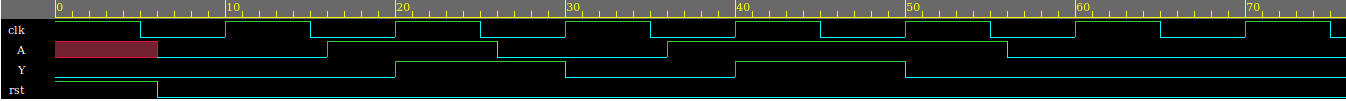
\includegraphics[width=450px,height=50px]{./assets/sequence_detector.png}
\end{center}
\subsubsection{Links}
\label{sec:org7f9cd30}

\href{https://www.edaplayground.com/x/3g3D}{Module}

\href{https://www.edaplayground.com/w/x/23g}{Waveform}
\subsection{Traffic Light Controller}
\label{sec:org83dd54c}
\subsubsection{TLC module}
\label{sec:org8eb812c}
\begin{enumerate}
\item Controller Module
\label{sec:orge831b44}
\begin{verbatim}
module traffic_light_controller(input TA, TB, clk, rst, output RA, YA, GA, RB, YB, GB);
  typedef enum logic [1:0] {S0,S1,S2,S3} statetype;
  statetype state, nextstate;
  always @ (posedge clk, posedge rst)
    if (rst) state <=  S0;
    else       state <= nextstate;
  always @ (*)
    case(state)
      S0: if (TA) nextstate = S0;
      else   nextstate = S1;
      S1:        nextstate = S2;
      S2: if (TB) nextstate = S2;
      else   nextstate = S3;
      S2:        nextstate = S0;
      default:   nextstate = S0;
    endcase
  // output logic
  assign RA = (state == S2 | state == S3);
  assign YA = (state == S1);
  assign GA = (state == S0);
  assign RB = (state == S0 | state == S1);
  assign YB = (state == S3);
  assign GB = (state == S2);
endmodule
\end{verbatim}
\item Sensor Module
\label{sec:org7f639f4}
\begin{verbatim}
module Traffic_sensor(T1, T2, clk, rst);
  output reg [4:0] T1, T2;
  input clk, rst;
  wire feedback1, feedback2;
  assign feedback1 = {(~(T1[4] ^ T1[3])),(~(T1[3] ^ T1[2]))};
  assign feedback2 = {(~(T1[4] ^ T1[3])),(~(T1[3] ^ T1[2]))};
  always @ (posedge clk, posedge rst)
    begin
      if (rst)
        begin
            T1 = 5'b01101;
            T2 = 5'b10110;
        end
      else
        begin
            T1 = {T1[2:0],feedback1};
            T2 = {T2[2:0],feedback2};
        end
    end
endmodule
\end{verbatim}
\end{enumerate}
\subsubsection{TLC Test Bench}
\label{sec:org21131c5}
\begin{enumerate}
\item Controller Test Bench (without sensor)
\label{sec:org29b8338}
\begin{verbatim}
`include "traffic_light_controller.vh"
module test_TLC();
  reg clk, rst;
  reg TA, TB;
  wire RA, YA, GA, RB, YB, GB;
  traffic_light_controller dut(TA,TB,clk,rst,RA,YA,GA,RB,YB,GB);
  always
    begin
      clk = 1; #5; clk = 0; #5;
    end
  initial begin
    rst = 1; #10; rst = 0;
    $display("Initially traffic in both lanes A and B");
    TA = 1; TB = 1; #10;
    $display("RA = %b, YA = %b, GA = %b", RA, YA, GA);
    $display("RB = %b, YB = %b, GB = %b\n", RB, YB, GB);
    #10;
    $display("RA = %b, YA = %b, GA = %b", RA, YA, GA);
    $display("RB = %b, YB = %b, GB = %b\n", RB, YB, GB);
    $display("----------------------");

    $display("Now traffic in A but not in B");
    TA = 1; TB = 0; #10;
    $display("RA = %b, YA = %b, GA = %b", RA, YA, GA);
    $display("RB = %b, YB = %b, GB = %b\n", RB, YB, GB);
    #10;
    $display("RA = %b, YA = %b, GA = %b", RA, YA, GA);
    $display("RB = %b, YB = %b, GB = %b\n", RB, YB, GB);
    $display("----------------------");

    $display("Now traffic in B but not in A");
    TA = 0; TB = 1; #10;
    $display("RA = %b, YA = %b, GA = %b", RA, YA, GA);
    $display("RB = %b, YB = %b, GB = %b\n", RB, YB, GB);
    #10;
    $display("RA = %b, YA = %b, GA = %b", RA, YA, GA);
    $display("RB = %b, YB = %b, GB = %b\n", RB, YB, GB);
    $display("----------------------");

    $display("Now traffic in neither");
    TA = 0; TB = 0; #10;
    $display("RA = %b, YA = %b, GA = %b", RA, YA, GA);
    $display("RB = %b, YB = %b, GB = %b\n", RB, YB, GB);
    #10;
    $display("RA = %b, YA = %b, GA = %b", RA, YA, GA);
    $display("RB = %b, YB = %b, GB = %b\n", RB, YB, GB);

  $finish;
end
endmodule
\end{verbatim}
\item Sensor Test Bench
\label{sec:org16e97fb}
\begin{verbatim}
`include "traffic_light_controller.vh"
module test_lfsr();
  reg clk, rst;
  wire [4:0] T;
  reg [4:0]  index;
  initial
    begin
        index = 4'b0;
        clk = 0;
        rst = 1;
        #15;
        rst = 0;
        #200;
    end
  always
    begin
        #5;
        clk = ~clk;
        index = index + 1;
        $display("T = %b", T);
        if(index === 5'b11111) begin
          $finish;
        end
    end
  Traffic_sensor dut(T,clk,rst);
endmodule
\end{verbatim}
\item Controller Test Bench (with sensor)
\label{sec:orge5d4c55}
\begin{verbatim}
`include "traffic_light_controller.vh"
module test_TLC();
  reg clk, rst;
  reg TA, TB;
  wire RA, YA, GA, RB, YB, GB;
  wire [4:0] A, B;
  Traffic_sensor input_string (A,B,clk,rst);
  traffic_light_controller dut(TA,TB,clk,rst,RA,YA,GA,RB,YB,GB);
  always
    begin
      clk = 1; #5; clk = 0; #5;
    end
  initial begin
    rst = 1; #10; rst = 0;
    TA = A[0]; TB = B[0]; #10;
    $display("Input String from Traffic Sensors:");
    $display("TA = %b; TB = %b\n", A, B);
    $display("RA = %b, YA = %b, GA = %b", RA, YA, GA);
    $display("RB = %b, YB = %b, GB = %b\n", RB, YB, GB);
    #10;
    $display("RA = %b, YA = %b, GA = %b", RA, YA, GA);
    $display("RB = %b, YB = %b, GB = %b\n", RB, YB, GB);
    $display("----------------------");

    TA = A[1]; TB = B[1]; #10;
    $display("RA = %b, YA = %b, GA = %b", RA, YA, GA);
    $display("RB = %b, YB = %b, GB = %b\n", RB, YB, GB);
    #10;
    $display("RA = %b, YA = %b, GA = %b", RA, YA, GA);
    $display("RB = %b, YB = %b, GB = %b\n", RB, YB, GB);
    $display("----------------------");

    TA = A[2]; TB = B[2]; #10;
    $display("RA = %b, YA = %b, GA = %b", RA, YA, GA);
    $display("RB = %b, YB = %b, GB = %b\n", RB, YB, GB);
    #10;
    $display("RA = %b, YA = %b, GA = %b", RA, YA, GA);
    $display("RB = %b, YB = %b, GB = %b\n", RB, YB, GB);
    $display("----------------------");

    TA = A[3]; TB = B[3]; #10;
    $display("RA = %b, YA = %b, GA = %b", RA, YA, GA);
    $display("RB = %b, YB = %b, GB = %b\n", RB, YB, GB);
    #10;
    $display("RA = %b, YA = %b, GA = %b", RA, YA, GA);
    $display("RB = %b, YB = %b, GB = %b\n", RB, YB, GB);
    $display("----------------------");

    TA = A[4]; TB = B[4]; #10;
    $display("RA = %b, YA = %b, GA = %b", RA, YA, GA);
    $display("RB = %b, YB = %b, GB = %b\n", RB, YB, GB);
    #10;
    $display("RA = %b, YA = %b, GA = %b", RA, YA, GA);
    $display("RB = %b, YB = %b, GB = %b\n", RB, YB, GB);

  $finish;
end
endmodule
\end{verbatim}
\end{enumerate}
\subsubsection{Timing}
\label{sec:org57ed8fb}
\begin{enumerate}
\item Waveform 1 (TLC without sensor)
\label{sec:org3c016d2}
\begin{center}
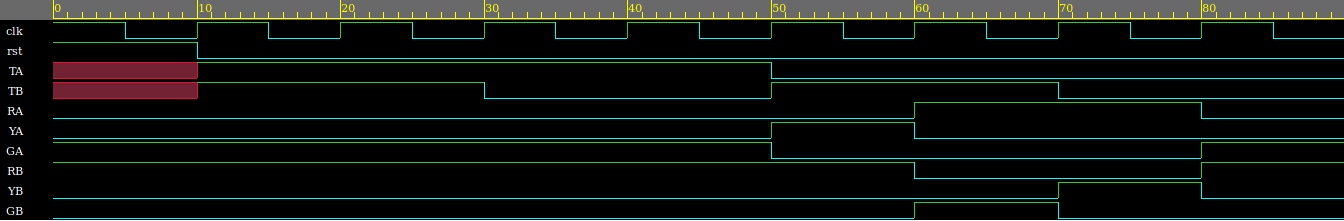
\includegraphics[width=450px,height=100px]{./assets/TLC_waveform1.png}
\end{center}
\item Waveform 2 (sensor)
\label{sec:orge85b38e}
\begin{center}
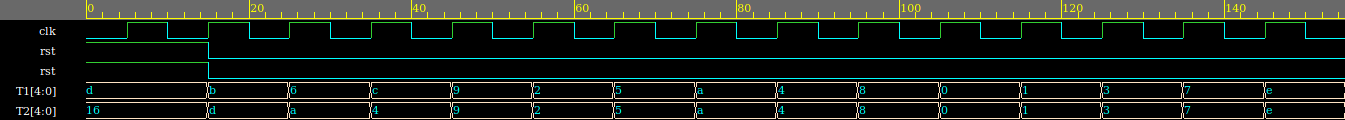
\includegraphics[width=450px,height=50px]{./assets/TLC_waveform2.png}
\end{center}
\item Waveform 3 (TLC with sensor)
\label{sec:org9a32f58}
\begin{center}
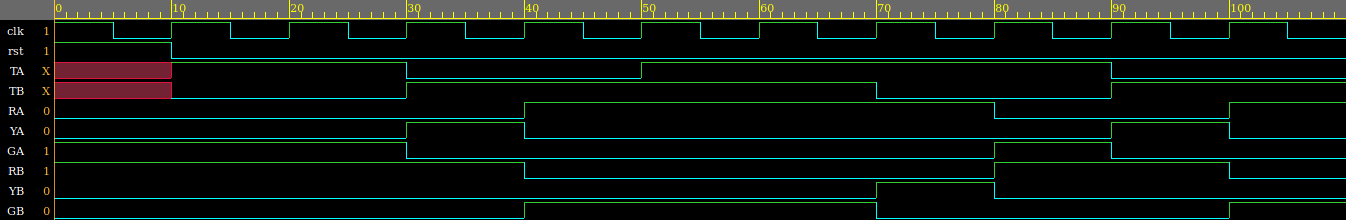
\includegraphics[width=450px,height=100px]{./assets/TLC_waveform3.png}
\end{center}
\end{enumerate}
\subsubsection{Links}
\label{sec:orgec42580}
\begin{enumerate}
\item Waveform 1 (TLC without sensor)
\label{sec:org65b540e}

\href{https://www.edaplayground.com/x/3qgC}{Module}

\href{https://www.edaplayground.com/w/x/2yK}{Waveform}
\item Waveform 2 (sensor)
\label{sec:org871b854}

\href{https://www.edaplayground.com/x/4vEy}{Module}

\href{https://www.edaplayground.com/w/x/3tx}{Waveform}
\item Waveform 3 (TLC with sensor)
\label{sec:org7b87b07}

\href{https://www.edaplayground.com/x/ie6}{Module}

\href{https://www.edaplayground.com/w/x/cy}{Waveform}
\end{enumerate}
\end{document}
